\documentclass[12pt]{article}

% Packages
\usepackage[margin=6em]{geometry} % 1 cm = 2.84528 em
\usepackage[colorlinks=true,linkcolor=red,urlcolor=blue]{hyperref}
\usepackage{tikz}
\usetikzlibrary{automata}
\usepackage[backend=bibtex]{biblatex}
\bibliography{sources}
\nocite{*}

\usepackage{lipsum}

% Paragraphs
\setlength{\parindent}{0em}
\setlength{\parskip}{1em}

% Includes
\input{antonxue-lib}


\let\company\undefined
\newcommand{\company}{\textbf{Big Tech Company}}

\let\Android\undefined
\newcommand{\android}{Android}

\let\state\undefined
\newcommand{\state}{\ensuremath{\sigma}}

\let\var\undefined
\newcommand{\var}{\ensuremath{x}}

\let\domval\undefined
\newcommand{\domval}{\ensuremath{\mathcal{A}}}

\let\formula\undefined
\newcommand{\form}{\ensuremath{\varphi}}

\let\domform\undefined
\newcommand{\domform}{\ensuremath{\mathcal{F}}}

% Author
\title{The Dangerous Graph}
\author{Anton Xue}
% \date{\today}
\date{}

% Document
\begin{document}
\maketitle

\subsection{Real-World Applications?}

A friend working at \company{} told to me about a problem
they were working on:
how do we automatically detect crashing errors in \android{} applications?

Users interacts with \android{} applications by touching
the phone's user interface (UI).
Touching the UI in specific ways alters the internal state of the application.
The UI is specified by XML files that (each?) represent a
different display layout.
When specific touches are performed, different displays may be shown.
These display transitions are conditional on the internal state of the
application and the current active display.

We then ask:
\textbf{what sequence of actions will cause the application to crash?}


\subsection{Defining the Problem}
From a high-level perspective, the problem is not well-defined in part
because we have not discussed the level of access we have to the
application under testing.
Are we given the source code?
Can we monitor internal application state and variables during execution?
Or are we given just the phone and told to play with it?

If we have access to the source code, we may apply techniques such as
backwards symbolic execution~\cite{baldoni-backwards} or
slicing~\cite{weiser-slicing}.

If we may monitor application state during execution through some debugger
or trace dumper, then short of decompilation, we may try techniques such
as randomized testing or somehow approximating behavior.

If we are given just a phone, then we throw it against a wall.

The first condition presented, with complete source code access, is of
course, the most favorable.
It is also the biggest headache because all the techniques listed are
a pain to implement.

We opt for the second.

\subsection{Modeling the Problem}
\begin{definition}[Application Graph]
An \textit{application graph} is a directed multigraph $G = \parens{V, E}$,
where each vertex $v \in V$ has a state $v_{\state}$ mapping
variables to a domain of values $\domval$,
and every edge $e = \parens{u, v}$ with tail $u$ and head $v$ is labeled
with a formula $e_{\form}$ in some logical theory $\domform$.
\end{definition}

The reason we define the application graph representation as a multigraph
is because program representation is hard.

Here, every vertex corresponds to some display, and we remark
that multiple vertices may exist that represents the same display.
For each vertex $v$, the state $v_{\state}$ is meant to map the variables
to a logical formula over their possible values as defined by their types.
This allows us to differentiate between the same display when, perhaps
the underlying state variable mappings differ.

Every edge represents an action, and for each edge $e$
the associated formula $e_{\form}$ is intended to capture the logical
conditions that must be satisfied when the action is performed in order
for the transition to occur.
We note that the conditions for edges that denote the same UI action
need not be mutually unsatisfiable.
This may be weird, and we attempt to address this later.
% This means that for any $u, v \in V$, all edges that have form
% $e = \parens{u, v}$ must have formulae such that
% $e_{i, \varphi}$ and $e_{j, \varphi}$ are not mutually satisfiable if
% $i \neq j$.
% Otherwise our transitions would be confusing.

So what does this all mean?

\begin{example}[Simple UI]
Testing the limits of our \LaTeX{} powers, we bring you this example.
Here, the application consists of three displays, each with tree elements:

\begin{itemize}
  \item
    A {\color{blue} blue $n$-value label} that shows the global value of $n$.

  \item
    A {\color{green} green action buton} that modifies $n$ according
    to its description.

  \item
    A {\color{red} red warp button} that moves between displays.
    Sometimes crashes.
\end{itemize}

I think the {\color{green} green color} actually hurts my eyes to read.

\begin{minipage}{0.45\textwidth}
  \begin{center}
  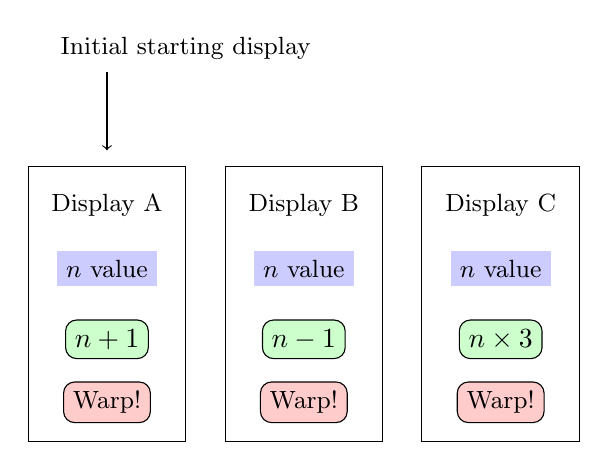
\begin{tikzpicture}
    \draw (0.0, 0.0) -- (2.0, 0.0) -- (2.0, 3.5) -- (0.0, 3.5) -- (0.0, 0.0);
    \draw (2.5, 0.0) -- (4.5, 0.0) -- (4.5, 3.5) -- (2.5, 3.5) -- (2.5, 0.0);
    \draw (5.0, 0.0) -- (7.0, 0.0) -- (7.0, 3.5) -- (5.0, 3.5) -- (5.0, 0.0);

    \node[] at (1.0, 3.0) {{\small Display A}};
    \node[] at (3.5, 3.0) {{\small Display B}};
    \node[] at (6.0, 3.0) {{\small Display C}};

    \node[fill=blue!20] at (1.0, 2.2) {{\small $n$ value}};
    \node[fill=blue!20] at (3.5, 2.2) {{\small $n$ value}};
    \node[fill=blue!20] at (6.0, 2.2) {{\small $n$ value}};

    \node[fill=green!20,draw,rounded corners] at (1.0, 1.3) {$n + 1$};
    \node[fill=green!20,draw,rounded corners] at (3.5, 1.3) {$n - 1$};
    \node[fill=green!20,draw,rounded corners] at (6.0, 1.3) {$n \times 3$};

    \node[fill=red!20,draw,rounded corners] at (1.0, 0.5) {{\small Warp!}};
    \node[fill=red!20,draw,rounded corners] at (3.5, 0.5) {{\small Warp!}};
    \node[fill=red!20,draw,rounded corners] at (6.0, 0.5) {{\small Warp!}};

    \node[] at (2.0, 5.0) {{\small Initial starting display}};

    \draw[->] (1.0, 4.7) -- (1.0, 3.7);

  \end{tikzpicture}
  \end{center}
\end{minipage}
\hfill
\begin{minipage}{0.5\textwidth}
\begin{pcode}
// Display A:
green: set n = n + 1
red:   if n mod 5 == 1 then go to B
       if n mod 5 == 2 then go to C
       otherwise do nothing
// Display B:
green: set n = n - 1
red:   if n mod 5 == 0 then go to A
       if n mod 5 == 2 then go to C
       otherwise do nothing
// Display C:
green: set n = n * 3
red:   if n mod 5 == 0 then go to A
       if n mod 5 == 1 then go to B
       otherwise CRASH
\end{pcode}
\end{minipage}

The state graph is then defined as follows:

{\color{red} \textbf{picture copied over from somewhere else; will fill in}}

\begin{center}
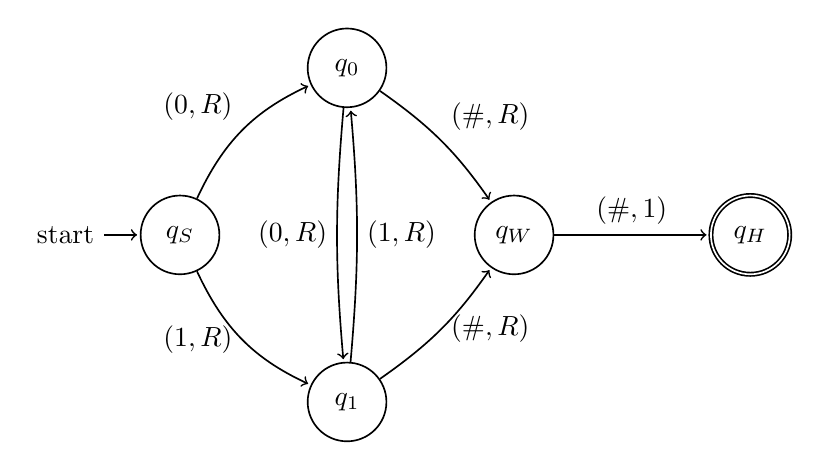
\begin{tikzpicture}
  [->,
   % >=stealth',
   shorten >=1pt,
   auto,
   node distance=3cm,
   semithick,
   state/.style={circle, draw, minimum size=1cm} 
  ]
  \node[state, initial]   (S)                    {$q_{S}$};
  \node[state]            (A) [above right of=S] {$q_{0}$};
  \node[state]            (B) [below right of=S] {$q_{1}$};
  \node[state]            (W) [below right of=A] {$q_{W}$};
  \node[state, accepting] (H) [right of=W]       {$q_{H}$};

  \path (S) edge [bend left=20] node
            {$(0, R)$} (A)
        (S) edge [bend right=20, left] node
            {$(1, R)$} (B)

        (A) edge [bend right=5, left] node
            {$(0, R)$} (B)
        (A) edge [bend left=10] node
            {$(\#, R)$} (W)
        
        (B) edge [bend right=5, right] node
            {$(1, R)$} (A)
        (B) edge [bend right=10, right] node
            {$(\#, R)$} (W)
        (W) edge [] node
            {$(\#, 1)$} (H)
        ;
\end{tikzpicture}
\end{center}



\end{example}


\subsection{The Dangerous Game}



\subsection{Conclusion}


\printbibliography


\end{document}
